% ######################################################################################################################
%         Introduction
% ######################################################################################################################

\chapter{Introduction}
\label{ch:Introduction}

% ######################################################################################################################
%         Background and Motivation
% ######################################################################################################################

\section{Background and Motivation}
\label{ch:Introduction:sec:Motivation}

The concept of evolution is the cornerstone of modern biology \cite{Dobzhansky1973}.
% \secref{ch:Foundations:sec:EvolutionGenetics}
All life on earth descends from a common ancestor and continuously evolves over generations,
which leads to a diversification of biological species.
The resulting branching pattern of the evolutionary relationships between species
is the key for unraveling many biological questions.
These evolutionary relationships are described by \emph{phylogenetic trees}
(\secref{ch:Foundations:sec:TreeOfLife}),
which are important in both basic \cite{Misof2014,Jarvis2014,Zanne2014} and
applied research \cite{Futuyma1995,Hendry2011,Schwartz2017}.

Characteristics and traits of biological species are inherited via their DNA
(\secref{ch:Foundations:sec:EvolutionGenetics}).
DNA data is hence often used for inferring a phylogenetic tree for a set of species
(\secref{ch:Foundations:sec:MLTreeInference}).
In order to conduct such analyses, the DNA has to be sequenced,
that is, it has to be ``read'' into some human-accessible format,
typically in form of a sequence of characters
(\secref{ch:Foundations:sec:SequenceAnalysis}).
In recent decades, the throughput of sequencing technologies increased,
while at the same time, the cost decreased faster than Moore's law,
as shown in \figref{fig:sequencing_costs}.
This lead to a ``tsunami'' of sequence data,
which constitutes a challenge for computational analyses of these data.
% computational biology

\begin{figure}[hbt]
    \centering
    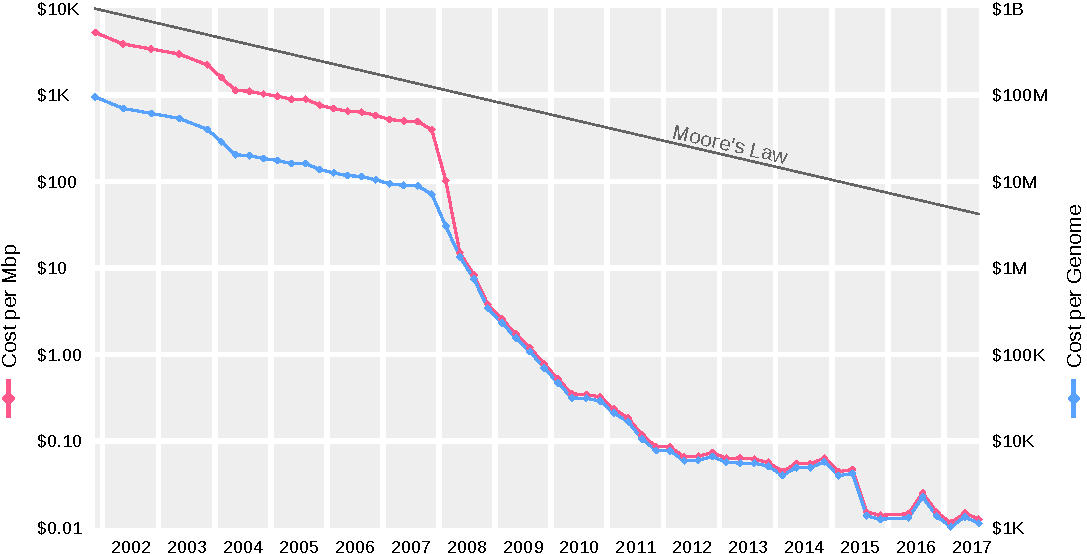
\includegraphics[width=\linewidth]{sequencing_costs.pdf}
    \caption[Sequencing costs per Mbp and per genome]{
        \textbf{Sequencing costs per Mbp and per genome.}
        The cost for DNA sequencing have decreased substantially in the past 15 years.
        The Figure shows the cost per mega-basepair (Mbp) of DNA (red line, left y-axis)
        as well as the cost per human-sized genome of $\approx$\,\num{3}\,Gbp (blue line, right y-axis).
        A basepair represents one character in the DNA.
        Note the logarithmic scaling of the y-axes.
        For comparison, Moore's law \cite{Moore1965} is shown.
        The particularly steep decrease in the beginning of 2008 is caused by
        the adoption of novel (next-generation) sequencing technologies in sequencing centers,
        see \secref{ch:Foundations:sec:SequenceAnalysis:sub:GenomeSequencing}.
        Source: Image based on data from \cite{Wetterstrand2018}.
%         \url{https://www.genome.gov/sequencingcosts/}
%         \url{https://www.genome.gov/sequencingcostsdata/}
    }
    \label{fig:sequencing_costs}
\end{figure}

In particular, these high-throughout technologies allow to directly sequence DNA contained in samples
that have been extracted from environments such as water, soil, or the human gut.
This results in so-called \emph{metagenomic} sequences,
i.e., anonymous DNA sequences from the (microbial) organisms that were present in the environmental sample.
A key question in the analysis of such data is to determine the evolutionary relationships of the sequences.
While these DNA sequences can hypothetically be used to infer phylogenetic trees from scratch,
this approach is limited by several theoretical and practical difficulties:
For instance, typical metagenomic samples contain too many, and too short, sequences
for a feasible and reliable tree inference.

One approach to tackle this issue is the so-called \emph{phylogenetic placement} \cite{Matsen2010,Berger2011},
of metagenomic sequences into a given phylogenetic tree (\secref{ch:Foundations:sec:PhylogeneticPlacement}).
Phylogenetic placement methods classify a set of \emph{query sequences}
into the context of known evolutionary relationships, provided in form of a \emph{reference tree}.
While this information already represents biological knowledge \emph{per se},
it can also be used for further downstream analyses \cite{Matsen2011a}.
The research in this field is however quite young and not many such analysis methods have been developed.

An important task prior to conducting phylogenetic placement of metagenomic sequences is to obtain a suitable
reference phylogenetic tree that captures the biological diversity of the species to be placed.
The assembly of a set of reference sequences from biological databases that can be used to infer such a tree
is typically a manual process, and hence both labor-intensive and potentially error-prone.
This might detain researchers from employing phylogenetic placement in the first place.

Furthermore, while the existing downstream methods for phylogenetic placement
(introduced in \secref{ch:Foundations:sec:PhylogeneticPlacement:sub:ExistingMethods})
allow for in-depth interpretation and visualization of the data,
they were not developed with a particular focus on large-scale studies comprising many thousand environmental samples.
For large datasets, these methods might provide too much detail,
making it hard to interpret results, to spot patterns and clusters in the data,
and to discover correlations with meta-data.

Lastly, the problem of scalability to large datasets does not only affect the methods themselves.
Because of the ever growing amount of sequence data,
scalability is becoming an issue for the software pipelines as well.
State-of-the-art phylogenetic placement implementations can place billions of sequences within a few hours \cite{Barbera2018}.
Methods for processing and analyzing the data, in particular phylogenetic placement data,
hence require efficient and scalable software implementations.

% ######################################################################################################################
%         Objective and Contribution
% ######################################################################################################################

\section{Objective and Contribution}
\label{ch:Introduction:sec:ObjectiveContribution}

in this thesis...

\chpref{ch:AutomaticTrees}

\chpref{ch:Visualization}

\chpref{ch:Clustering}

we developed methods for working with such data, and helped to conduct several empirical studies using established as well as our novel methods.

method papers (main contrib for this work, see next section)
phat \cite{Czech2018}
vis clust \cite{Czech2018a}



tree viz review \cite{Czech2017}



method and software dev:

salt \cite{Flouri2017}

unieuk \cite{Berney2017}

tree clustering workshop?

epa ng \cite{Barbera2018}

quartet score \cite{Zhou2017}

swarm code contrib \cite{Mahe2014,Mahe2015}

scrapp




data analysis:

1kite \cite{Misof2014}
\url{http://1kite.org}

neotrop \cite{Mahe2017}

microsopirida \cite{Bass2018a}

long reads (in prep)

dinos (in prep)




mention genesis and gappa, their implementation chapter in the appendix,
their paper?!
github links
\url{https://github.com/lczech/genesis}
\url{https://github.com/lczech/gappa}

genesis: implements some established methods, just way faster

mention  \url{http://github.com/lczech/placement-methods-paper} for the result files of two of the papers

full list of publications is available in \secref{ch:Publications}

% ######################################################################################################################
%         Structure and Overview
% ######################################################################################################################

\section{Structure and Overview}
\label{ch:Introduction:sec:StructureOverview}


\todo{check that the url and access date of all online sources are present in bibliography!}

% \todo{I used a few public domain images from wikipedia as sources, and modified them as needed. make sure that this is okay.}

\todo{search for all abbreviations used and add them to the acro list. also, check Pierre's MA, and Alexey's and Andre's Diss for needed acronyms!}
\todo{list of acronyms!} see andre, add MB/GB, PCA,
BV, TO, HMP, etc

\todo{unify table and figure caption capitalization}

\todo{more workflow flow charts?}
